% !TEX root = DesignDocument.tex


\chapter{Research Results}

%%This chapter describes the results and conclusions of your research.   This would be the final report for a research project.  

By the conclusion of the project, many different results had been drawn about several aspects of the cluster. The first are the results of testing of each single device. Then, the maximum amount of Gigaflops the cluster can produce with LINPACK was found. GPIO and USB communication were also analyzed. 

\section{Result 1}

First, the Raspberry PI 2B and ODROID XU4 were tested individually to find which was faster. The results are shown in Figure~\ref{pivodroid} along with the final metric of Gigaflops per dollar per watt. It was found that the Raspberry Pi cost \$35 and used 4 watts of power while running, and the ODroid cost \$75 and used 15 watts. 

\begin{figure}[tbh]
\begin{center}
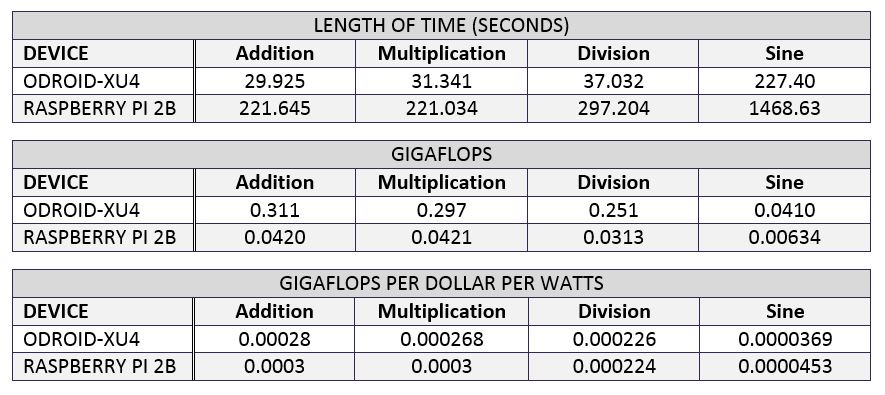
\includegraphics[width=0.75\textwidth]{pivsxu4table2.JPG}
\end{center}
\caption{PI vs ODROID results. \label{pivodroid}}
\end{figure}

\section{Result 2}

We also measured the speed of the Ethernet connections using the tool iperf. It was testing by directly connecting two devices Ethernet to Ethernet, and connected over the switch. Also, using USB to Etherent devices to create new network interfaces on the ODroids was tested by connecting those ports to the built in Ethernet ports. The results are shown in Table~\ref{ethernet}

\begin{table}[tbh]
\caption{Ethernet speeds. \label{ethernet}}
\begin{center}
\begin{tabular}{|r|l|}
  \hline
  Ethernet to Ethernet & 750 Mbps \\
  USB to Ethernet &  450 Mbps \\ 
  Ethernet over switch & 750 Mbps \\
  \hline
\end{tabular}
\end{center}
\end{table}

\section{Result 3}

Direct USB to USB communication was also tested. The devices were attached by USB 3.0 ports with the intent to use them to pass information between. However, further research proved that there is no current way to transfer information from two hosts using USB 3.0. It can be done with USB 2.0 using crossover cables, but there does not exist any common operating system that supports the same feature with 3.0. Therefore, we did not benchmark USB 3.0 communication.

\section{Result 4}

Another alternate form of communication tested was GPIO. The library WiringPi was installed and used with C to read and write values to pins. It was found that communication was successful, but in order to make a protocol faster than Ethernet, even if we used all 40 pins to tranfer data, we would need each pin to send over 19.5 million bits per second, as per \begin{equation}(750 * 1024^{2}) / 40 \end{equation}WiringPi, in our preliminary testing, was only able to send about 500,000 bits per second on a pin. Therefore, it was concluded that our cluster would always be faster using Ethernet.

\section{Result 5}

Our final result was using LINPACK to test the amount of Gigaflops produced by the cluster. 

\begin{figure}[tbh]
\begin{center}
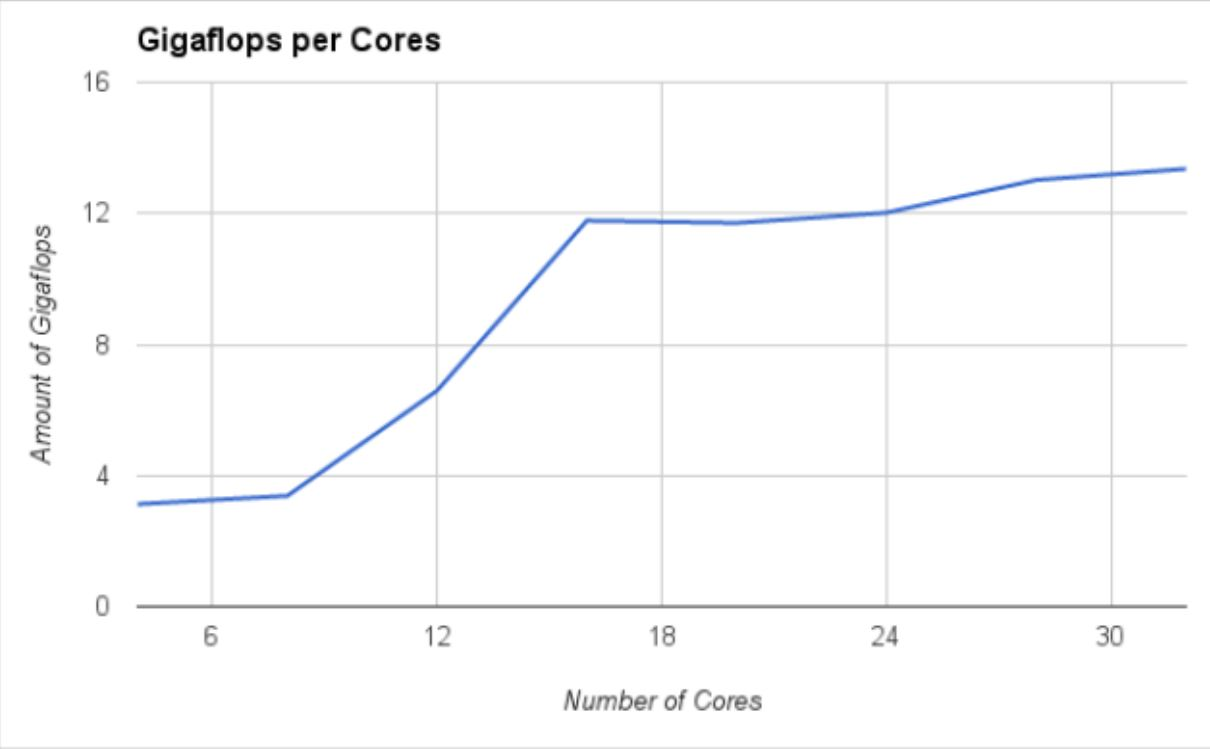
\includegraphics[width=0.75\textwidth]{minimalgraph.JPG}
\end{center}
\caption{LINPACK results. \label{linpackresults}}
\end{figure}

\section{Conclusions}

\section{Further work}  
